\subsubsection{Nanoscience and catalysis }
\index{Richards, Ryan}

\paragraph{Research Team}
Dr. Ryan Richards (Professor),
 Andreas Suchopar (Lab manager/technician)
Dr. Juncheng Hu (Postdoctoral researcher) Zhi Li (Phd student)
Lifang Chen (Phd student) Divakara SG (Phd student) Bener
Yeginoglu (MS student) Upakul Deka (MS student)
\\

%150 words about research in general

The interface of the fields of catalysis and nanoscale materials
is one of the most exciting areas of modern science and is at the
forefront of the quest for a sustainable future.  The field of
nanotechnology has generated a great deal of interest primarily
because on this size scale numerous new and potentially useful
properties have been observed including: melting point, specific
heat, surface reactivities, catalytic, magnetic, and optical
properties.

The impact of catalysis in our current everyday lives cannot be
understated. It was recently estimated that 35 \% of global GDP
depends on catalysis. In addition the goal of sustainability with
regard to energy and environmental concerns will most certainly
require significant contributions from catalysis.

A three-fold approach is being pursued in the Richards' laboratory
to establish an understanding of nanoscale materials: 1)
preparation of nanomaterials (metals and metal oxides) with a
controlled size, shape and composition then combining these
materials via the 'precursor' concept to form composites; 2)
characterization of the physical and chemical properties as a
function of size, shape and composition; and 3) examination of the
factors that influence the stability of the nanoscale materials
and their properties (particularly catalysis).

\paragraph{Highlights}

%500 words about highlights in 2006

The major accomplishments of 2006 were: (1) discovery of a novel
wet-chemical approach to preparing MgO with the polar 111 surface
IUB-Z, (2) preparation of a mesoporous silica containing gold
nanoparticles within the walls, (3) anchoring of man-made chiral
ligands onto metallic surfaces to induce enantioselectivity, and
(4) the immobilization of several polyoxometalate species on high
surface area metal oxides to form very active oxidation catalysts.
\begin{enumerate}
\item In recent years, theoretical physicists have predicted that
the 111 plane of MgO could be stable and may possess very
interesting properties.  However, to date, MgO possessing the 111
plane has never been prepared.  Recently, in the Richards'
laboratory, we discovered a direct method for the preparation of
this material. This preparation is currently the subject of a
submitted patent and publication in the highest impact chemistry
journal Angewandte Chemie whereby it is named IUB-Z MgO. \item
Gold nano-particles confined in the walls of mesoporous silica
(GMS) catalysts were successfully prepared by a novel and simple
technique utilizing thioether functional groups in the walls of
mesoporous silica to anchor HAuCl4. Calcination of the materials
removed organic moieties and reduced the gold salt to gold
nanoparticles. In this procedure, the thioether groups were
introduced into the silica wall via a co-condensation of
tetraethyl orthosilicate (TEOS) with 1,4-bis(triethoxysily)propane
tetrasulfide. These gold containing mesoporous catalysts have
unusually high surface area and pore volume. The catalysts
demonstrated exceptional activity for the oxidation of benzyl
alcohol under relatively mild conditions. \item Platinum modified
with cinchonidine have been employed as 'quasi-homogeneous'
catalysts for the hydrogenation of ethyl pyruvate and have
demonstrated exceptional activities while the ee's of these
systems are currently inferior to the traditional $Pt/Al_2O_3$
heterogeneous system. Using DRIFTS (Diffuse Reflectance Infra-red
Fourier Transform Spectroscopy) analysis of samples together with
geometry optimization and IR modelling we have studied the
orientation of cinchonidine on Pt and Fe nanoclusters and
additionally the man-made ligand quiphos on Pt nanoclusters. It
has been determined that cinchonidine can adsorb on Pt and Fe
nanoclusters in both 'flat' and 'tilted' modes, while quiphos can
be adsorbed on Pt only via the 'p-bonded' mode. Further studies in
this area have demonstrated that the chiral ligand DIOP can also
be employed as a modifier that induces chirality. In addition,
recent studies have shown that dramatically different interactions
between the metal and modifier exist when Pd is used. These
studies thus provide an insight into modifier orientation on
nanocluster surfaces that can be extended to a wide range of
potential modifiers and facilitate a better understanding of the
origin of enantioselectivity with these 'quasi-homogeneous'
catalyst systems. \item The aerobic oxidation of saturated
hydrocarbons into the corresponding ketones and alcohols is
potentially important for the petrochemical and fine chemical
industries. There are only a few examples for these oxidations
found in the literature because of problems associated with
catalyst deactivation and difficulty of C-H bond/$O_2$ activation.
Thus, the most desirable approach to alkane oxidation would be to
use a heterogeneous catalyst in combination with air under solvent
free conditions. To reach these objectives, iron-substituted
polyoxometalates (Fe-POMs) were immobilized on
3-aminopropyltriethoxysilane (apts) modified SBA-15. These
combined POM/mesoporous silica systems showed excellent catalytic
performance for solvent-free aerobic oxidation of long chain
n-alkanes using air as the oxidant under ambient conditions
through a classical free radical chain autoxidation mechanism.
This work is especially important as it establishes a field of
research at IUB that cannot be matched elsewhere because it
combines the expertise of Prof. Kortz (synthesis of novel poms)
with the expertise of our group in preparing nanoparticles and
applying them in catalytic reactions.
\end{enumerate}

% Pictures are to be included via:

\begin{figure}[ht]
  \begin{center}
    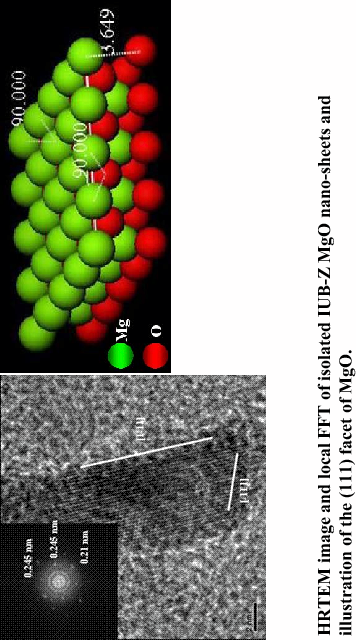
\includegraphics[height=\hsize, angle=270]{Richards/Richards_2006_Fig.png}
    \mycaption{ HRTEM image and local FFT of isolated IUB-/
    MgO nano sheets and illustration of the (111) facet of MgOP)}\label{fig:Richards 2006 Fig}
   \end{center}
\end{figure}



\paragraph{Collaborations}
The group maintains an international collaboration within the
framework of the EU COST D-24 project focused on the preparation
of novel heterogeneous enantioselective catalysts with groups from
Slovenia, Romania, Belgium, France and Sweden as well as
initiatives with industrial partners (confidential).  Finally,
there are numerous collaborations ongoing and developing with IUB
colleagues (Profs. Kortz, Nugent, Nau, Materny and Tautz).



\paragraph{Grants}
% list the running grants in 2005, if none have been received, please delete this
% subsection.
\begin{enumerate}
\item Funded by EU COST D24 working group, \emph{Heterogeneous Enantioselective Catalysis}
  (2002 - 2006)
\item Funded by confidential industrial partner (Co-PI with Ulrich Kortz) 100,000 euro,
  2005
\item Funded by confidential industrial partner (Co-PI with Ulrich Kortz) 200,000 euro,
  (2006 - 2007)
\item Funded by confidential industrial partner 102,000 euro, 2007 
\end{enumerate}


\paragraph{Patens}
% list the grants you have received in 2005, if none have been received, please delete this
% subsection.
\begin{enumerate}
\item US patent (US20021) filed February 17, 2006; Kake Zhu,
Christian Kuebel, Ryan Richards; ''Nanosheets of MgO Possessing
the 111 Plane and Method of Manufacturing the same.'' \item 1
additional patent filed in April with confidential industrial
partner.
\end{enumerate}

%Publications should be delivered as a separate file (naming
%convention profxxx.bib. See description by R. Helling. Please make
%sure that all your publications are referred to in the TiX file.
%This can either be in form of a \cite{profxxxkey} or as a
%\nocite{profxxxkey} in the end. A publication which is not
%reffered to on the LaTeX file doesn't produce any output in the
%report.
\nocite{Richards1}
\nocite{Richards2}
\nocite{Richards3}
\nocite{Richards4}
\nocite{Richards5}
\nocite{Richards6}
\nocite{Richards7}
\nocite{Richards8}
\nocite{Richards9}
\nocite{Richards10}
\nocite{Richards11}
\nocite{Richards12}
